\documentclass[dvipsnames, aspectratio=169]{beamer}
\usepackage[utf8]{inputenc}
\usepackage{listings}
\usepackage{comment}
\usepackage{soul}
%\usepackage{ulem}
\usepackage{subfig}
\usepackage{pgf-pie}
\setul{}{1pt}
\usepackage[oldenum, olditem]{paralist}
%allow even smaller text
\newcommand\tinytiny{\fontsize{4pt}{3}\selectfont}

\makeatletter
\let\old@lstKV@SwitchCases\lstKV@SwitchCases
\def\lstKV@SwitchCases#1#2#3{}
\makeatother
\usepackage{lstlinebgrd}
\makeatletter
\let\lstKV@SwitchCases\old@lstKV@SwitchCases

\lst@Key{numbers}{none}{%
    \def\lst@PlaceNumber{\lst@linebgrd}%
    \lstKV@SwitchCases{#1}%
    {none:\\%
     left:\def\lst@PlaceNumber{\llap{\normalfont
                \lst@numberstyle{\thelstnumber}\kern\lst@numbersep}\lst@linebgrd}\\%
     right:\def\lst@PlaceNumber{\rlap{\normalfont
                \kern\linewidth \kern\lst@numbersep
                \lst@numberstyle{\thelstnumber}}\lst@linebgrd}%
    }{\PackageError{Listings}{Numbers #1 unknown}\@ehc}}
\makeatother


\usepackage{tikz}
\graphicspath{{4_0/figures/}}
%disclaimer for Sandia. uncomment and the whole blob goes away @ b80c116300122
\def\sandid{SANDXXXX PE}

% \title{Performance Portability with Kokkos}
\title{Kokkos 4.3 Release Briefing}

%BAD misuse of author field
\author{New Capabilities}


\usetheme{kokkos}

\newif\ifshort
\newif\ifmedium
\newif\iffull
\newif\ifnotoverview

\newcommand{\TutorialDirectory}{\texttt{Intro-Full}}
\newcommand{\ExerciseDirectory}[1]{\texttt{Exercises/#1/}}
\newcommand{\TutorialClone}{\texttt{Kokkos/kokkos-tutorials/\TutorialDirectory}}

\definecolor{darkgreen}{rgb}{0.0, 0.5, 0.0}
\definecolor{darkred}{rgb}{0.8, 0.0, 0.0}
\definecolor{orange}{rgb}{0.8, 0.33, 0.0}
\definecolor{purple}{rgb}{0.60, 0.20, 0.80}
\colorlet{bodyColor}{blue!20}
\colorlet{patternColor}{orange!30}
\colorlet{policyColor}{green!30}

% http://tex.stackexchange.com/questions/144448/color-a-text-line-in-a-code-lstlisting
\lstnewenvironment{code}[1][]%
{
  %with txfonts: OT1/txr/m/n/10
  %with default fonts: OT1/cmr/m/n/10
  %\fontfamily{cmr}\selectfont
  %\showthe\font
   \noindent
   \minipage{\linewidth}
   %\vspace{0.5\baselineskip}
   \lstset{mathescape, escapeinside={<@}{@>},
moredelim=**[is][{\btHL[fill=patternColor]}]{@pattern}{@pattern},
moredelim=**[is][{\btHL[fill=red!30]}]{@warning}{@warning},
moredelim=**[is][{\btHL[fill=policyColor]}]{@policy}{@policy},
moredelim=**[is][{\btHL[fill=bodyColor]}]{@body}{@body},
moredelim=**[is][{\btHL[fill=red!30]}]{@warning}{@warning},
moredelim=**[is][\color{black}]{@black}{@black},
moredelim=**[is][\color{blue}]{@blue}{@blue},
moredelim=**[is][\bf]{@bold}{@bold},
moredelim=**[is][\it]{@italic}{@italic},
moredelim=**[is][\color{boldblue}\bf]{@boldblue}{@boldblue},
moredelim=**[is][\color{red}]{@red}{@red},
moredelim=**[is][\color{green}]{@green}{@green},
moredelim=**[is][\color{gray}]{@gray}{@gray},
moredelim=**[is][\color{darkgreen}]{@darkgreen}{@darkgreen},
moredelim=**[is][\color{darkred}]{@darkred}{@darkred},
moredelim=**[is][\color{orange}]{@orange}{@orange},
moredelim=**[is][\color{purple}]{@purple}{@purple},
keywords={},
#1}
}
{
  \endminipage
  %\vspace{1.0\baselineskip}
}

\makeatletter
\newif\ifATOlinebackground
\lst@Key{linebackground}{\tiny}{\def\ATOlinebackground{#1}\global\ATOlinebackgroundtrue}
\makeatother

\lstnewenvironment{shell}[1][]{%
  \global\ATOlinebackgroundfalse
  \lstset{language=sh,%
    showstringspaces=false,
    aboveskip=0pt,
    frame=none,
    numbers=none,
    belowskip=2pt,
    breaklines=true,
    #1,
    }
  %\ifATOlinebackground
  \lstset{linebackgroundcolor={
    \ATOlinebackground
  }}
  %\fi
  }{}

\lstnewenvironment{cmake}[1][]{%
  \global\ATOlinebackgroundfalse
  \lstset{language=sh,%
    showstringspaces=false,
    aboveskip=0pt,
    frame=none,
    numbers=none,
    belowskip=2pt,
    breaklines=true,
    #1,
    }
  %\ifATOlinebackground
  \lstset{linebackgroundcolor={
    \ATOlinebackground
  }}
  %\fi
  }{}

\newcommand{\inlinecode}[1]{{\lstset{basicstyle=\ttfamily,keywordstyle={},showstringspaces=false}\lstinline$#1$}}
\newcommand{\inlineshell}[1]{{\lstset{basicstyle=\ttfamily,keywordstyle={},showstringspaces=false}\lstinline$#1$}}

\setbeamercolor{block title}{fg=white, bg=SandiaLightBlue}
\setbeamercolor{block body}{bg=lightgray}
\setbeamercolor{block title alerted}{fg=white, bg=SandiaRed}
\setbeamercolor{block body alerted}{bg=lightgray}



%\usepackage[texcoord,grid,gridunit=mm,gridcolor=red!10,subgridcolor=green!10]{eso-pic}
\usepackage[absolute,overlay]{textpos}





% http://tex.stackexchange.com/questions/8851/how-can-i-highlight-some-lines-from-source-code

\usepackage{pgf, pgffor}
\usepackage{listings}
\usepackage{lstlinebgrd} % see http://www.ctan.org/pkg/lstaddons

\makeatletter
%%%%%%%%%%%%%%%%%%%%%%%%%%%%%%%%%%%%%%%%%%%%%%%%%%%%%%%%%%%%%%%%%%%%%%%%%%%%%%
%
% \btIfInRange{number}{range list}{TRUE}{FALSE}
%
% Test in int number <number> is element of a (comma separated) list of ranges
% (such as: {1,3-5,7,10-12,14}) and processes <TRUE> or <FALSE> respectively

\newcount\bt@rangea
\newcount\bt@rangeb

\newcommand\btIfInRange[2]{%
    \global\let\bt@inrange\@secondoftwo%
    \edef\bt@rangelist{#2}%
    \foreach \range in \bt@rangelist {%
        \afterassignment\bt@getrangeb%
        \bt@rangea=0\range\relax%
        \pgfmathtruncatemacro\result{ ( #1 >= \bt@rangea) && (#1 <= \bt@rangeb) }%
        \ifnum\result=1\relax%
            \breakforeach%
            \global\let\bt@inrange\@firstoftwo%
        \fi%
    }%
    \bt@inrange%
}
\newcommand\bt@getrangeb{%
    \@ifnextchar\relax%
        {\bt@rangeb=\bt@rangea}%
        {\@getrangeb}%
}
\def\@getrangeb-#1\relax{%
    \ifx\relax#1\relax%
        \bt@rangeb=100000%   \maxdimen is too large for pgfmath
    \else%
        \bt@rangeb=#1\relax%
    \fi%
}

%%%%%%%%%%%%%%%%%%%%%%%%%%%%%%%%%%%%%%%%%%%%%%%%%%%%%%%%%%%%%%%%%%%%%%%%%%%%%%
%
% \btLstHL<overlay spec>{range list}
%
% TODO BUG: \btLstHL commands can not yet be accumulated if more than one overlay spec match.
%
\newcommand<>{\btLstHL}[2]{%
  \only#3{\btIfInRange{\value{lstnumber}}{#1}{\color{#2}\def\lst@linebgrdcmd{\color@block}}{\def\lst@linebgrdcmd####1####2####3{}}}%
}%
\makeatother






% http://tex.stackexchange.com/questions/15237/highlight-text-in-code-listing-while-also-keeping-syntax-highlighting
%\usepackage[T1]{fontenc}
%\usepackage{listings,xcolor,beramono}
\usepackage{tikz}

\makeatletter
\newenvironment{btHighlight}[1][]
{\begingroup\tikzset{bt@Highlight@par/.style={#1}}\begin{lrbox}{\@tempboxa}}
{\end{lrbox}\bt@HL@box[bt@Highlight@par]{\@tempboxa}\endgroup}

\newcommand\btHL[1][]{%
  \begin{btHighlight}[#1]\bgroup\aftergroup\bt@HL@endenv%
}
\def\bt@HL@endenv{%
  \end{btHighlight}%
  \egroup
}
\newcommand{\bt@HL@box}[2][]{%
  \tikz[#1]{%
    \pgfpathrectangle{\pgfpoint{1pt}{0pt}}{\pgfpoint{\wd #2}{\ht #2}}%
    \pgfusepath{use as bounding box}%
    \node[anchor=base west, fill=orange!30,outer sep=0pt,inner xsep=1pt, inner ysep=0pt, rounded corners=3pt, minimum height=\ht\strutbox+1pt,#1]{\raisebox{1pt}{\strut}\strut\usebox{#2}};
  }%
}
\makeatother



\usetikzlibrary{calc}
\usepackage{xparse}%  For \NewDocumentCommand

% tikzmark command, for shading over items
\newcommand{\tikzmark}[1]{\tikz[overlay,remember picture] \node (#1) {};}

\makeatletter
\NewDocumentCommand{\DrawBox}{s O{}}{%
    \tikz[overlay,remember picture]{
    \IfBooleanTF{#1}{%
        \coordinate (RightPoint) at ($(left |- right)+(\linewidth-\labelsep-\labelwidth,0.0)$);
    }{%
        \coordinate (RightPoint) at (right.east);
    }%
    \draw[red,#2]
      ($(left)+(-0.2em,0.9em)$) rectangle
      ($(RightPoint)+(0.2em,-0.3em)$);}
}

\NewDocumentCommand{\DrawBoxWide}{s O{}}{%
    \tikz[overlay,remember picture]{
    \IfBooleanTF{#1}{%
        \coordinate (RightPoint) at ($(left |- right)+(\linewidth-\labelsep-\labelwidth,0.0)$);
    }{%
        \coordinate (RightPoint) at (right.east);
    }%
    \draw[red,#2]
      ($(left)+(-\labelwidth,0.9em)$) rectangle
      ($(RightPoint)+(0.2em,-0.3em)$);}
}

\NewDocumentCommand{\DrawBoxWideBlack}{s O{}}{%
    \tikz[overlay,remember picture]{
    \IfBooleanTF{#1}{%
        \coordinate (RightPoint) at ($(left |- right)+(\linewidth-\labelsep-\labelwidth,0.0)$);
    }{%
        \coordinate (RightPoint) at (right.east);
    }%
    \draw[black,#2]
      ($(left)+(-\labelwidth,0.9em)$) rectangle
      ($(RightPoint)+(0.2em,-0.3em)$);}
}
\makeatother

\usetikzlibrary{positioning}

\usetikzlibrary{shapes}

\hypersetup{
    colorlinks=true,
    linkcolor=blue,
    filecolor=magenta,
    urlcolor=cyan,
}



\shorttrue
\mediumfalse
\fullfalse

\begin{document}

\begin{frame}
        \titlepage
\end{frame}


\begin{frame}[fragile]{Outline}

\textbf{4.3 Release Highlights}

    \begin{itemize}
      \item{Organizational}
      \item{Backend updates}
      \item{Build system updates}
      \item{\texttt{Kokkos::sort\_by\_key}}
      \item{Miscellaneous}
      \item{Deprecations and other breaking changes}
    \end{itemize}

\end{frame}

\begin{frame}{Find More}

\textbf{Online Resources}:

\begin{itemize}
        \item \url{https://github.com/kokkos}:
                \begin{itemize}
                        \item Primary Kokkos GitHub Organization
                \end{itemize}
        \item \url{https://github.com/kokkos/kokkos-tutorials/wiki/Kokkos-Lecture-Series}:
                \begin{itemize}
			\item{Slides, recording and Q\&A for the Full Lectures}
                \end{itemize}
        \item \url{https://kokkos.github.io/kokkos-core-wiki}:
                \begin{itemize}
                        \item Wiki including API reference
                \end{itemize}
        \item \url{https://kokkosteam.slack.com}:
                \begin{itemize}
                        \item Slack channel for Kokkos.
                        \item Please join: fastest way to get your questions answered.
                        \item Can whitelist domains, or invite individual people.
                \end{itemize}
\end{itemize}

\end{frame}

\begin{frame}[fragile]{Kokkos Usage}
  \textbf{Would like to strengthen community bonds and discoverability}

\vspace{10pt}
\textit{List of Applications and Libraries}
\begin{itemize}
\item Add your app to \url{https://github.com/kokkos/kokkos/issues/1950}
\item We are planning to add that to a Kokkos website.
\item Helps people discover each other when working on similar things.
\end{itemize}

\vspace{10pt}
\textit{GitHub Topics}
\begin{itemize}
\item Use \textit{kokkos} tag on your repos.
\item If you click on the topic you get a list of all projects on github with that topic.
\end{itemize}

\end{frame}

\begin{frame}[fragile]{Kokkos Topic}
  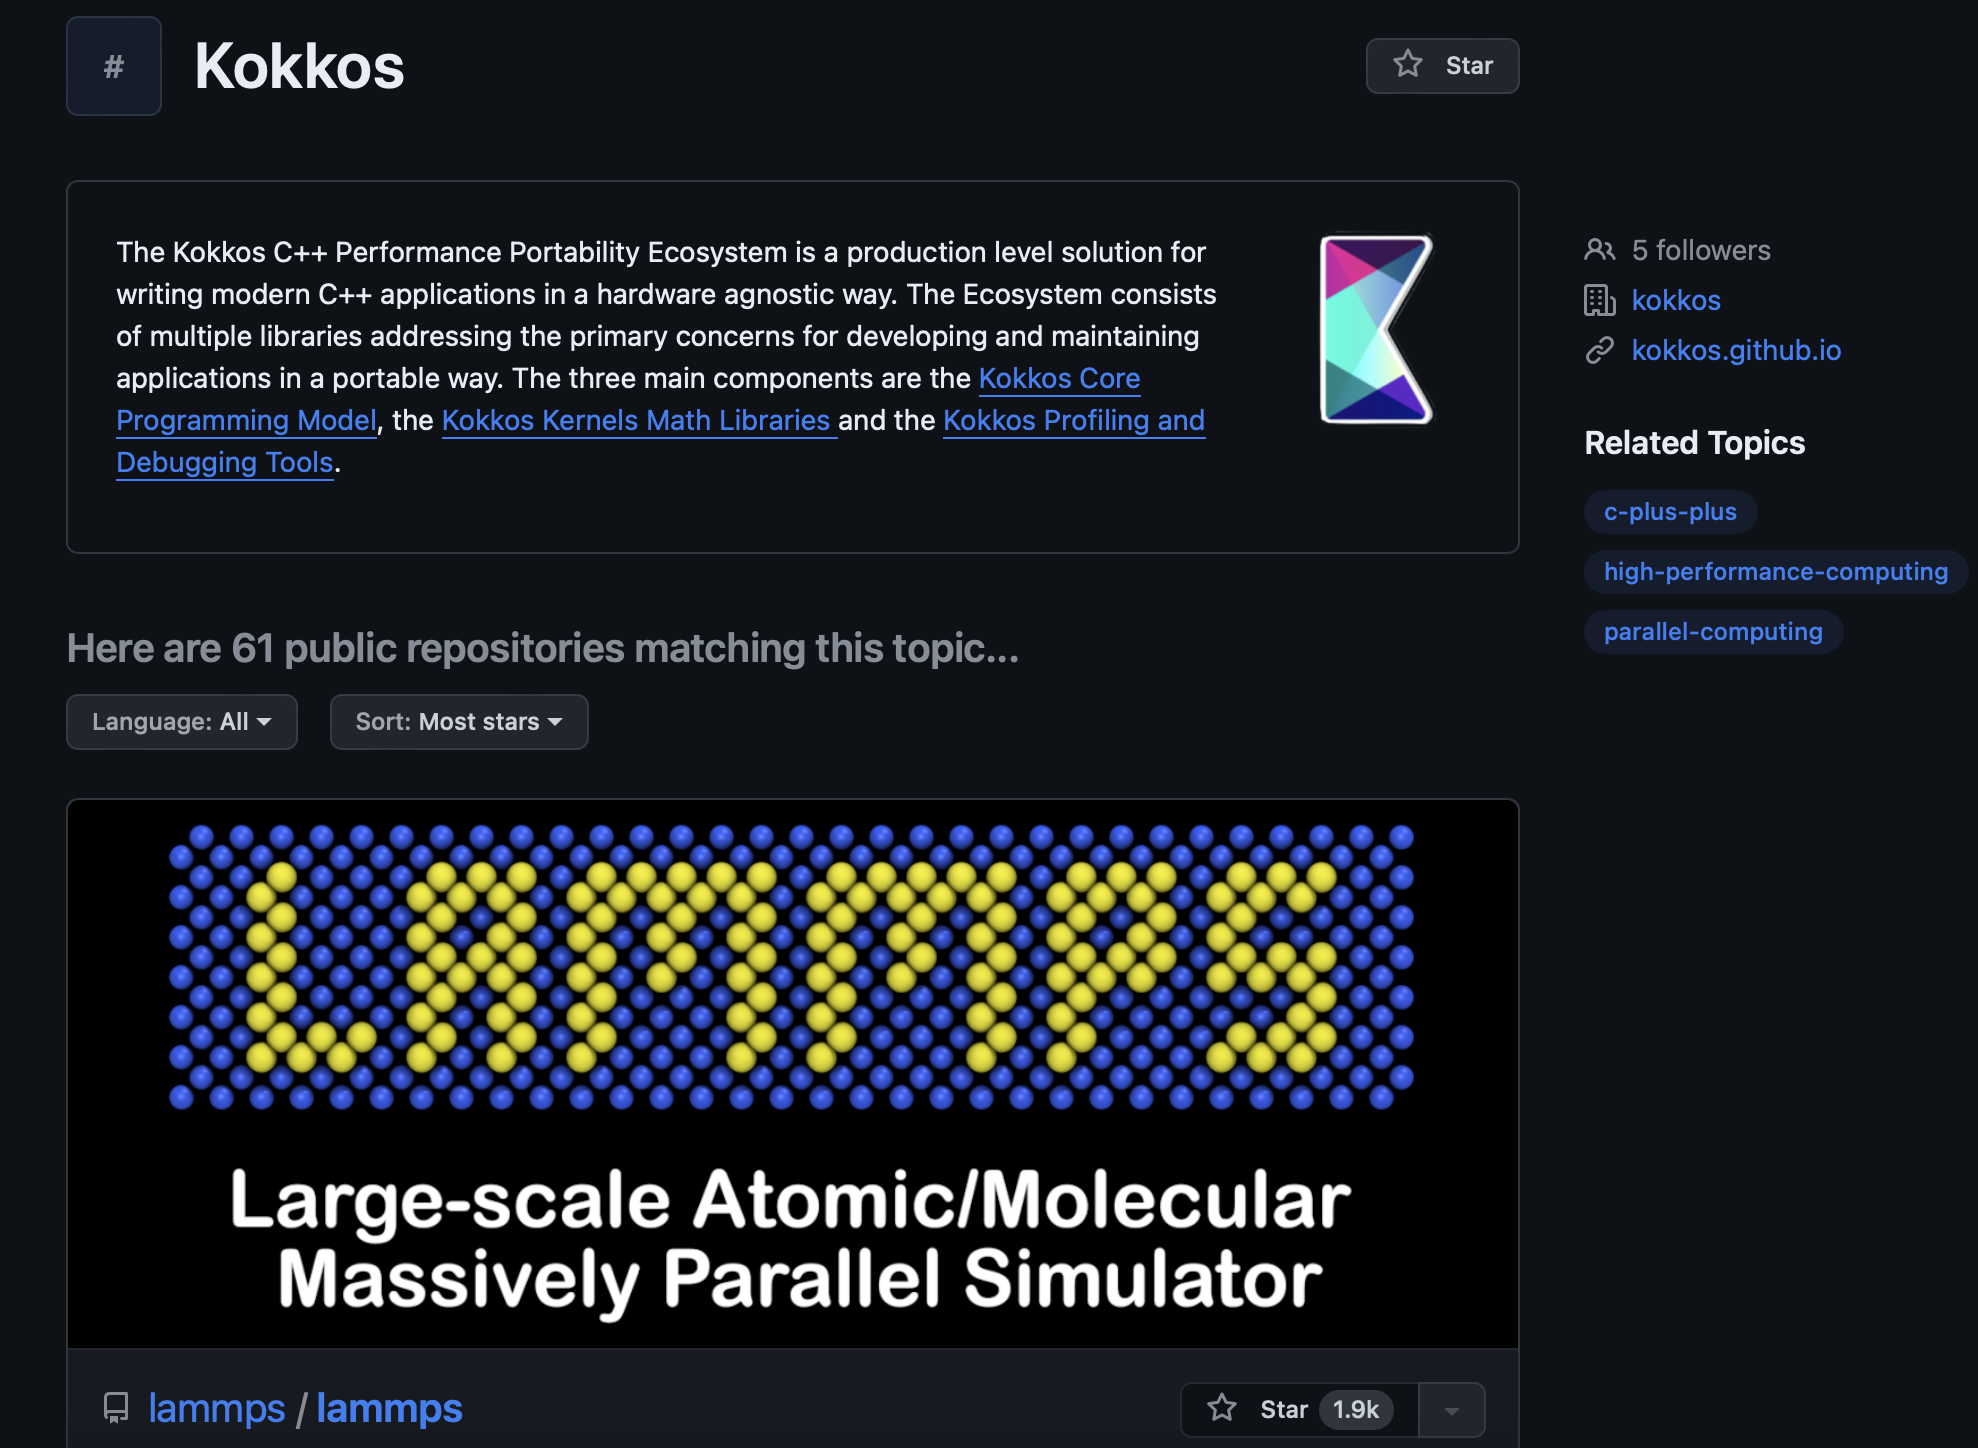
\includegraphics[width=0.9\textwidth]{4_3/kokkos-topic}
\end{frame}


%==========================================================================

\begin{frame}[fragile]

  {\Huge Organizational}

  \vspace{10pt}

  \textbf{Content:}
  \begin{itemize}
    \item HPSF and Kokkos Meeting 2025
    \item Targetting C++20 for Kokkos 5.0
    \item SequentialHostInit and Views of Views 
  \end{itemize}

\end{frame}

%==========================================================================

\begin{frame}[fragile]{Kokkos User Group Meeting 2025}
\begin{center}
\textbf{Kokkos User Group Meeting 2025 @ HPSF Conference}
\end{center}

\begin{itemize}
\item{\textit{When:} May 5th-8th 2025}
\item{\textit{Where:} Chicago}
\item{\textit{What:} 2-days HPSF plenary + 2-days Project meetings}
\item{\textit{KUG-Content Request:} Focused on user experiences
\begin{itemize}
   \item{How do you leverage Kokkos?}
   \item{What are pain points?}
   \item{Kokkos based libraries of interest for the community}
\end{itemize}
}
\end{itemize}


\vspace{10pt}

\begin{center}
\textit{Registration will open in January!}
\end{center}
\end{frame}


\begin{frame}[fragile]{Kokkos 5 and ISO C++20}
\begin{center}
\textbf{Kokkos 5 is comming Summer 2025}

\vspace{0.5cm}
\textbf{We will require C++20!}
\end{center}

\textit{Start preparing now:}
\begin{itemize}
  \item{Check availability of compilers on your systems}
  \item{Test with C++20 enabled: start with a CPU build}
  \item{Minimum Compiler requirements will change (more details later)}
\end{itemize}

\vspace{0.5cm}
\begin{center}
\textit{Nothing wrong for your project to require C++20 now if you feel ready!}
\end{center}
\end{frame}


%==========================================================================

\begin{frame}[fragile]

  {\Huge Backend Updates}

  \vspace{10pt}

\end{frame}


%==========================================================================

% Examples

% note: always keep the [fragile] for your frames!

%\begin{frame}[fragile]{Title}
%  Contents
%\end{frame}

%==========================================================================
\begin{frame}[fragile]{CUDA and SYCL}
  \begin{itemize}
    \item CUDA: Add support for AMPERE87 architecture (Jetson Orin Nano)
    \item CUDA: Support RDC with Clang 17+ and use new offload driver
    \item SYCL: Add support for Intel DG2 GPUs such as the Arc Alchemist GPUs
    \item SYCL: Allow using non-trivially-copyable comparators with oneDPL
  \end{itemize}
\end{frame}

%==========================================================================

\begin{frame}[fragile]{Improve half float performance for CUDA and SYCL backends}
  \begin{itemize}
    \item CUDA AND SYCL: Directly use the available fp16 mathematical function instead of casting back and forth to fp32
  \end{itemize}
  \begin{tikzpicture}
    \begin{axis}[
        width  = 0.85*\textwidth,
        height = 0.75*\textheight,
        major x tick style = transparent,
        ybar=2*\pgflinewidth,
        bar width=14pt,
        ymajorgrids = true,
        ylabel = {Exec time (µs)},
        symbolic x coords={Memory Bound Kernel, Compute Bound Kernel},
        xtick = data,
        scaled y ticks = false,
        enlarge x limits=0.25,
        ymin=0,
        legend style={at={(0.3,0.75)},anchor=west},
    ]
        \addplot
            coordinates {(Memory Bound Kernel, 32) (Compute Bound Kernel, 102)};

        \addplot
            coordinates {(Memory Bound Kernel, 15.8) (Compute Bound Kernel, 102)};

        \addplot
            coordinates {(Memory Bound Kernel, 14.7) (Compute Bound Kernel, 63)};

        \legend{float 32, fp16 old, fp16 new}
    \end{axis}
\end{tikzpicture}
\end{frame}

% Bench details:
% - NVidia A100
% - 2^20 (1 million) elements
% - Memory bound kernel is doing:
% tmp = init(i);
% res(i) = sqrt(cos(tmp) + sin(tmp));
% - Compute bound is doing 16 time the work of Memory Bound

%==========================================================================

\begin{frame}[fragile]{OpenMPTarget}
  \begin{itemize}
      \item Remove support for non-llvm compilers as part of the strategy to only support LLVM compilers in the backend.
      \item LLVM compilers support extensions to OpenMP directives on GPU that allow \textit{grid} style kernel launches making it more suitable for GPUs and avoiding the overhead of OpenMP's fork-join model.
  \end{itemize}
\end{frame}

%==========================================================================

%==========================================================================

\begin{frame}[fragile]

  {\Huge Build Systems Updates}

  \vspace{10pt}

\end{frame}

%==========================================================================

% Examples

% note: always keep the [fragile] for your frames!

\begin{frame}[fragile]{New build system features}
  \begin{itemize}
    \item Add support for Zen 4 AMD microarchitecture (\texttt{Kokkos\_ARCH\_ZEN4})
    \item Enable NVIDIA Grace architecture with NVHPC (\texttt{Kokkos\_ARCH\_ARMV9\_GRACE})
    \item Support static library builds via \texttt{CMAKE\_CUDA\_RUNTIME\_LIBRARY=static} when using CUDA as CMake language
  \end{itemize}

\end{frame}

%==========================================================================


%==========================================================================


%==========================================================================

\begin{frame}[fragile]{sort\_by\_key}

\textbf{Introduced sort\_by\_key to dispatch to optimized vendor libraries}

\vspace{10pt}

\begin{code}
  ExecutionSpace exec_space;
  Kokkos::View<int*> keys("keys", n);
  Kokkos::View<float*> values("values", n);
  Kokkos::Experimental::sort_by_key(exec_space, keys, values);
\end{code}

\vspace{10pt}

\begin{itemize}
  \item 1D views only
  \item Sizes of \texttt{keys} and \texttt{values} must match
  \item Both \texttt{keys} and \texttt{values} are modified
  \item Dispatches to vendor libraries (Thrust, rocThrust, oneDPL) when available
\end{itemize}

\end{frame}

%==========================================================================


%==========================================================================

\begin{frame}[fragile]

  {\Huge General Enhancements}

  \vspace{10pt}

\end{frame}

%==========================================================================

% Examples

% note: always keep the [fragile] for your frames!

\begin{frame}[fragile]{Architecture Support and Performance}
 \begin{itemize}
     \item Support for AMD Zen 5, SiFive RISC-V Y74MC and ARMv8.4 CPU architectures
     \begin{itemize}
       \item new \texttt{KOKKOS\_ARCH\_AMD\_ZEN5} 
       \item new \texttt{KOKKOS\_ARCH\_RISCV\_U74MC}
     \end{itemize}
     \item {Resolving performance regression with atomic views for HIP and SYCL}
     \begin{itemize}
       \item \texttt{atomic\_op\_fetch} now always use vendor APIs for atomics (e.g. \texttt{sycl\_atomic\_ref})
     \end{itemize}
     \item Passing label~\emph{by reference} in all Kokkos Tools APIs (improving performance)
 \end{itemize}
\end{frame}

\begin{frame}[fragile]{APIs and Behaviours}
 \begin{itemize}
   \item Exit early at initialize with \texttt{--kokkos-help}
    \begin{itemize}
      \item Calling ``\texttt{binary --kokkos-help}" now causes normal termination
   \end{itemize}  
   \item Enable structured binding of return values for \texttt{partition\_space}
        \begin{code}[keywords={std}]
          /* NEW! */
          auto [exec0, exec1] = 
                  Experimental::partition_space(ExecSpace, 1, 1);
        \end{code}
    \item Avoid static variables and functions in header
    \begin{itemize}
      \item  Ensures compatibility with C++20 modules
      \end{itemize}
    \item Add \texttt{constexpr} specifier to \texttt{operator==} and \texttt{operator!=} for \texttt{Kokkos::complex}
    \item Add constructors for \texttt{Random\_XorShift*\_Pool} with execution space argument
      \begin{itemize}
      \item Allows construction of instances with non-blocking initialization
    \end{itemize}

 \end{itemize}
\end{frame}

\begin{frame}[fragile]{APIs and Behaviours (Continued)}
 \begin{itemize}
     \item Add \texttt{Kokkos::SIMD::SVE} support for 128-bit and 256-bit SVE 
     \begin{itemize}
      \item Adds support for \emph{Scalable Vector Extensions} for Kokkos SIMD types on ARM V8.4-compatible CPUs
      \item Enabled with~\texttt{KOKKOS\_ARCH\_NATIVE}, ~\texttt{KOKKOS\_ARCH\_ARM\_SVE} and
 ~\texttt{KOKKOS\_ARCH\_ARMV9\_GRACE}
     \end{itemize}
     \item Implement \texttt{Kokkos::nextafter} for fp16 types
        \begin{code}[keywords={std}]
          /* NEW! */
          using half_t = Kokkos::Experimental::half_t;
          half_t a = 1.0, t = 2.0;
          half_t b = Kokkos::nextafter(a, t);
        \end{code}
        \item Removes~\texttt{[[nodiscard]]} attributes from the Kokkos SIMD interface to align with C++26
 \end{itemize}
\end{frame}


\begin{frame}[fragile]{Updates on Kokkos Graphs}
 \begin{itemize}
     \item Reminder: \emph{Kokkos Graph} is an abstraction of computation represented as a DAG
     \item Located in~\emph{Kokkos::Experimental}
      \item Example of a diamond-shaped compute graph supported
      \begin{code}[keywords={std}]
      auto graph = Kokkos::create_graph([&](auto root) {
      auto nodeA = root.then_parallel_for("workloadA",policy,functor);
      auto nodeB = nodeA.then_parallel_for("workloadB",policy,functor);
      auto nodeC = nodeA.then_parallel_for("workloadC",policy,functor);
      auto nodeD = Kokkos::when_all(nodeB, nodeC).
        then_parallel_for("workloadD",policy,functor);});
      graph.instantiate();
      graph.submit();
      \end{code}
     \item Restricted to Kokkos parallel patterns!
 \end{itemize}
\end{frame}


\begin{frame}[fragile]{Updates on Kokkos Graphs (Capture)}
 \begin{itemize}
     \item Add support for graph capture (Cuda, HIP and SYCL)
     \begin{itemize}
     \item Graph capture allows to add a graph node containing device code or library
     \item Supported backends: HIP, CUDA, SYCL (\emph{*\_capture})
  \end{itemize}
     \item Example: Capture of a cuBLAS call:
        \begin{code}[keywords={std}]
    auto graph = Kokkos::Experimental::create_graph([&](const auto& root){
      auto handle = create_cublas_handle();
       /* NEW! */
      root.cuda_capture(exec,
      [=](const Kokkos::Cuda& exec_){
        /* Body of lambda using CUDA */
        cublasSetStream(handle.get(),exec_.cuda_stream()));
        cublasDgemv( handle.get(),CUBLAS_OP_N,...);
      });
    });
    graph.instantiate(); 
    graph.submit(exec);
      \end{code}
     
 \end{itemize}
\end{frame}


\begin{frame}[fragile]{Updates on Kokkos Graphs (then\_host)}
 \begin{itemize}
     \item Add support for host-side graph nodes via the \emph{then\_host(...)} function
     \begin{itemize}
     \item Adding a host-node creates a new CPU execution node and adds it to the graph
     \item Registers a host-callback (and fences device exec space on execution)
  \end{itemize}
 \item Example: Using a host-side graph node
        \begin{code}[keywords={std}]
    const counter_t counter(Kokkos::view_alloc("counter", exec));
    ASSERT_EQ(counter.use_count(), 1);
      auto graph = Kokkos::Experimental::create_graph(exec, 
        [&](const auto& root) {
          root.then ("NodeA",exec,functor_d_t{{counter}})
          /* NEW!*/
          .then_host("NodeB",     functor_h_t{{counter}}) 
          .then     ("NodeC",exec,functor_d_t{{counter}});
      });
      ASSERT_EQ(counter.use_count(), 4);
      \end{code}
  \begin{itemize}
  \item Note:\emph{exec} can access host memory
  \end{itemize}
 \end{itemize}

\end{frame}

\begin{frame}[fragile]{Updates on Kokkos Graphs (other)}
 \begin{itemize}
    \item Allow building Kokkos::Experimental::Graph object directly
    \begin{itemize}
    \item Allows default-constructed Kokkos::Experimental::Graph 
    \item Graph has a new \emph{root\_node()} public member function (returns the graph's root node)
    \item Example use:
     \begin{code}[keywords={std}]
      /* NEW! */
      Kokkos::Experimental::Graph graph{exec};
      graph.root_node().then_parallel_for(1, func{});
      graph.submit(exec);
        \end{code}
     \end{itemize}
  \item Enforce unit launch bound for graph \emph{then-node}
  \begin{itemize}
    \item Now we explicitly use an execution policy with Kokkos::LaunchBounds<1> to execute a \emph{then} graph node
  \end{itemize}
 \end{itemize}
\end{frame}


%\begin{frame}[fragile]{Example code}
%    \begin{code}[keywords={std}]
%        #include <iostream>
%        
%        int main() {
%            std::cout << "hello world\n";
%        }
%    \end{code}
%\end{frame}

%\begin{frame}[fragile]{Example table}
%    \begin{center}
%        \begin{tabular}{l|l}
%            a & b \\\hline
%            c & d
%        \end{tabular}
%    \end{center}
%\end{frame}

%==========================================================================

%==========================================================================


%==========================================================================

\begin{frame}[fragile]

  {\Huge Querying the Number of Devices}

  \vspace{10pt}

	\textbf{Content:}
  \begin{itemize}
    \item Runtime function for querying the number of devices
    \item Device ID consistency with \texttt{KOKKOS\_VISIBLE\_DEVICES}
  \end{itemize}

\end{frame}

%==========================================================================

\begin{frame}[fragile]{Querying the number of devices}

\textbf{A runtime function to query the number of devices}
\bigskip

\texttt{[[nodiscard]] int Kokkos::num\_devices() noexcept {...}}
\vspace{10pt}

\begin{itemize}
	\item Callable before \texttt{Kokkos::initialize()}
	\item Returns the device count based on visible devices
	\item Returns -1 if no GPU backend is enabled
	\item Replaces \texttt{{Cuda,HIP}::detect\_device\_count()}
\end{itemize}

\end{frame}

%==========================================================================

\begin{frame}[fragile]{Kokkos::device\_id() consistency}

\textbf{Fixed a defect in \texttt{Kokkos::device\_id()}}
\bigskip

\texttt{KOKKOS\_VISIBLE\_DEVICES} were not being considered for \texttt{Kokkos::device\_id()}.
\vspace{10pt}

\begin{table}[]
\begin{tabular}{l|llll}
\multicolumn{1}{c|}{\textbf{initialization settings}} & \multicolumn{1}{c}{\textbf{Pre-4.3}} & \multicolumn{1}{c}{\textbf{4.3}} &  &  \\ \hline
\textless{}none\textgreater{}                         & 0                                    & 0                                &  &  \\
device\_id=1                                          & 1                                    & 1                                &  &  \\
KOKKOS\_VISIBLE\_DEVICES=0                            & 0                                    & 0                                &  &  \\
KOKKOS\_VISIBLE\_DEVICES=3                            & 3                                    & 0                                &  &  \\
KOKKOS\_VISIBLE\_DEVICES=1,0                          & 1                                    & 0                                &  &  \\
device\_id=1 KOKKOS\_VISIBLE\_DEVICES=1,0             & 0                                    & 1                                &  & 
\end{tabular}
\end{table}

\end{frame}

%==========================================================================


%==========================================================================

\begin{frame}[fragile]

  {\Huge Kokkos SIMD}

  \vspace{10pt}

  \textbf{Content:}
	\begin{itemize}
		\item \texttt{simd\_flags}
		\item \texttt{vector\_aligned\_tag}
	\end{itemize}

\end{frame}

%==========================================================================

\begin{frame}[fragile]{simd\_flags}

\textbf{Introduced \texttt{simd\_flags} to match latest ISO C++ proposal on \texttt{std::simd}}

\vspace{10pt}

\texttt{template <typename... Flags> struct simd\_flags}

\vspace{10pt}

\begin{itemize}
	\item \texttt{element\_aligned\_tag <-> simd\_flag\_default}
	\item \texttt{vector\_aligned\_tag <-> simd\_flag\_aligned}
\end{itemize}

\vspace{10pt}
\texttt{simd\_flags} are used in:
\begin{itemize}
  \item \texttt{template <class U, class Flags> void copy\_from(const U* mem, Flags flags)}
  \item \texttt{template <class U, class Flags> void copy\_to(U* mem, Flags flags)}
\end{itemize}

\end{frame}

%==========================================================================

\begin{frame}[fragile]{simd\_flags}

\begin{code}[keywords={simd_flags}]
void init_var() {
  constexpr size_t alignment =
    Kokkos::Experimental::native_simd::size() * sizeof(DataType);

  alignas(alignment) DataType const src[N] = { ... };

  simd_type var;
  var.copy_from(src, Kokkos::Experimental::simd_flag_aligned);

  ...
}
\end{code}

\end{frame}

%==========================================================================

%==========================================================================

\begin{frame}[fragile]

  {\Huge Bitset Constructor Update}

\end{frame}

%==========================================================================

\begin{frame}[fragile]{Bitset constructor update}

\texttt{Bitset(unsigned arg\_size = 0u)}
\vspace{10pt}
\begin{itemize}
	\item A \texttt{Bitset} constructor with a default size of \texttt{Bitset} was making a deferred constructor call.
	\item Caused an unnecessary memory allocation when \texttt{Bitset} was constructed with the default size of 0.
\end{itemize}

\vspace{10pt}

Refactored to no longer have the default argument and use a defaulted default \texttt{Bitset} constructor instead.

\end{frame}

%==========================================================================

%==========================================================================

\begin{frame}[fragile]

  {\Huge Random Number Generator}

\end{frame}


\begin{frame}[fragile]{Random Number Generator}
\texttt{Normal distribution improvements}
\begin{itemize}
\item Replace Marsaglia polar method with Box-Muller method 
\item Box-Muller contains no branching/looping, single code path, ideal for GPU
\item Kokkos performance on GPU, Nvidia: 
\begin{itemize}
\item ~20\% faster for 64 bit version
\item ~60\% faster for 1024 bit version
\end{itemize}
\end{itemize}
\end{frame}

%==========================================================================


%==========================================================================

\begin{frame}[fragile]

  {\Huge New Public Headers}
  
    \vspace{10pt}

  \textbf{Content:}
    \begin{itemize}
        \item \texttt{Kokkos\_Clamp.hpp}
        \item \texttt{Kokkos\_MinMax.hpp}
    \end{itemize}


\end{frame}

%==========================================================================

\begin{frame}[fragile]{Kokkos\_Clamp.hpp}

\begin{code}[keywords={Clamp}]

// bounded value

template<class T>
constexpr const T& clamp(const T& value, const T& low, const T& high);

template<class T, class ComparatorType>
constexpr T const& clamp(const T& value, const T& low, const T& high,
                         ComparatorType comp);

\end{code}

\end{frame}

%==========================================================================

\begin{frame}[fragile]{Kokkos\_MinMax.hpp Max}

\begin{code}[keywords={MinMax}]

// max

template <class T>
constexpr const T& max(const T& a, const T& b);
  
template <class T, class ComparatorType>
constexpr const T& max(const T& a, const T& b, ComparatorType comp);
  
template <class T>
constexpr T max(std::initializer_list<T> ilist); 
      
template <class T, class Compare>
constexpr T max(std::initializer_list<T> ilist, Compare comp); 


\end{code}

\end{frame}

%==========================================================================
\begin{frame}[fragile]{Kokkos\_MinMax.hpp Min}

\begin{code}[keywords={MinMax}]

// min

template <class T>
constexpr const T& min(const T& a, const T& b);

template <class T, class ComparatorType>
constexpr const T& min(const T& a, const T& b,ComparatorType comp);

template <class T>
constexpr T min(std::initializer_list<T> ilist);

template <class T, class Compare>
constexpr T min(std::initializer_list<T> ilist, Compare comp);

\end{code}

\end{frame}

%==========================================================================
\begin{frame}[fragile]{Kokkos\_MinMax.hpp MinMax}

\begin{code}[keywords={MinMax}]

// minmax

// minmax
template <class T>
constexpr Kokkos::pair<const T&, const T&> minmax(const T& a, const T& b);

template <class T, class ComparatorType>
constexpr Kokkos::pair<const T&, const T&> minmax(const T& a, const T& b,
                                                  ComparatorType comp);

template <class T>
constexpr Kokkos::pair<T, T> minmax(std::initializer_list<T> ilist);

template <class T, class Compare>
constexpr Kokkos::pair<T, T> minmax(std::initializer_list<T> ilist, Compare comp);

\end{code}

\end{frame}

%==========================================================================


%==========================================================================

\begin{frame}[fragile]

  {\Huge Compile-Time Argument Deduction (CTAD / Deduction Guides)}
  
    \vspace{10pt}

  \textbf{Content:}
    \begin{itemize}
        \item What are deduction guides?
        \item \texttt{Kokkos::Array} deduction guide
        \item \texttt{Kokkos::RangePolicy} deduction guides
        \item \texttt{Kokkos::MDRangePolicy} deduction guides
    \end{itemize}


\end{frame}

%==========================================================================

\begin{frame}[fragile]{CTAD / Deduction Guides}

\begin{itemize}
\item C++17
\item Usability Improvement
\item Deduces class template parameters from types and/or number of parameters passed to constructors
\item Eliminates need to specify template parameters when declaring automatic variables
\end{itemize}

\end{frame}

%==========================================================================

\begin{frame}[fragile]{Array Deduction Guide}

\begin{code}[keywords={Array}]
// Kokkos::Array<double, 3>
Kokkos::Array a4{3.0, 1.0, 4.0};	
\end{code}

\begin{itemize}
\item matches \texttt{std::array} deduction guide
\end{itemize}

\end{frame}

%==========================================================================

\begin{frame}[fragile]{RangePolicy Deduction Guides}

\begin{code}[keywords={RangePolicy}]

int64_t work_begin   = /* ... */;  // conversions as well
int64_t work_end     = /* ... */;  // conversions as well
Kokkos::ChunkSize cs = /* ... */;  // conversions as well
Kokkos::DefaultExecutionSpace des; // conversions as well
SomeExecutionSpace ses;            // different from Kokkos::DefaultExecutionSpace

// Kokkos::RangePolicy<>
Kokkos::RangePolicy rp0;
Kokkos::RangePolicy rp1(work_begin, work_end);
Kokkos::RangePolicy rp2(work_begin, work_end, cs);
Kokkos::RangePolicy rp3(des, work_begin, work_end);
Kokkos::RangePolicy rp4(des, work_begin, work_end, cs);

// Kokkos::RangePolicy<SomeExecutionSpace>
Kokkos::RangePolicy rp5(ses, work_begin, work_end);
Kokkos::RangePolicy rp6(ses, work_begin, work_end, cs);

\end{code}

\end{frame}

%==========================================================================

\begin{frame}[fragile]{MDRangePolicy initializer\_list Deduction Guides}

\begin{code}[keywords={MDRangePolicy initializer_list}]

Kokkos::DefaultExecutionSpace des;
SomeExecutionSpace ses;            // different from Kokkos::DefaultExecutionSpace
int64_t i;

// Kokkos::MDRangePolicy<Kokkos::Rank<5>>
Kokkos::MDRangePolicy pl0({1, 2, 3, 4, 5}, {1, 2, 3, 4, 5});
Kokkos::MDRangePolicy pl1({1, 2, 3, 4, 5}, {1, 2, 3, 4, 5}, { i });
Kokkos::MDRangePolicy pl2(des, {1, 2, 3, 4, 5}, {1, 2, 3, 4, 5});
Kokkos::MDRangePolicy pl3(des, {1, 2, 3, 4, 5}, {1, 2, 3, 4, 5}, { i });

// Kokkos::MDRangePolicy<SomeExecutionSpace, Kokkos::Rank<5>>
Kokkos::MDRangePolicy pl4(ses, {1, 2, 3, 4, 5}, {1, 2, 3, 4, 5});
Kokkos::MDRangePolicy pl5(ses, {1, 2, 3, 4, 5}, {1, 2, 3, 4, 5}, { i });

\end{code}

\end{frame}

%==========================================================================

\begin{frame}[fragile]{MDRangePolicy C Array Deduction Guides}

\begin{code}[keywords={MDRangePolicy C Array}]

Kokkos::DefaultExecutionSpace des;
SomeExecutionSpace ses;            // different from Kokkos::DefaultExecutionSpace
int cbegin[3];
int cend[3];
int64_t ctiling[2];

// Kokkos::MDRangePolicy<Kokkos::Rank<3>>
Kokkos::MDRangePolicy pc0(cbegin, cend);
Kokkos::MDRangePolicy pc1(cbegin, cend, ctiling);
Kokkos::MDRangePolicy pc2(des, cbegin, cend);
Kokkos::MDRangePolicy pc3(des, cbegin, cend, ctiling)

// Kokkos::MDRangePolicy<SomeExecutionSpace, Kokkos::Rank<3>>
Kokkos::MDRangePolicy pc4(ses, cbegin, cend);
Kokkos::MDRangePolicy pc5(ses, cbegin, cend, ctiling);

\end{code}

\end{frame}

%==========================================================================
\begin{frame}[fragile]{MDRangePolicy Array Deduction Guides}

\begin{code}[keywords={MDRangePolicy Kokkos::Array}]

Kokkos::DefaultExecutionSpace des;
SomeExecutionSpace ses;            // different from Kokkos::DefaultExecutionSpace
Kokkos::Array<int, 2> abegin;
Kokkos::Array<int, 2> aend;
Kokkos::Array<int64_t, 2> atiling;

// Kokkos::MDRangePolicy<Kokkos::Rank<2>>
Kokkos::MDRangePolicy pa0(abegin, aend);
Kokkos::MDRangePolicy pa1(abegin, aend, atiling);
Kokkos::MDRangePolicy pa2(des, abegin, aend);
Kokkos::MDRangePolicy pa3(des, abegin, aend, atiling)

// Kokkos::MDRangePolicy<SomeExecutionSpace, Kokkos::Rank<2>>
Kokkos::MDRangePolicy pa4(ses, abegin, aend);
Kokkos::MDRangePolicy pa5(ses, abegin, aend, atiling);

\end{code}

\end{frame}

%==========================================================================

%==========================================================================

\begin{frame}[fragile]

  {\Huge Misc. Algorithmic Improvements/Fixes}

\end{frame}

\begin{frame}[fragile]{Misc. Algorithmic Improvements/Fixes}
\begin{itemize}
\item Kokkos\textunderscore Unique.hpp
\begin{itemize}
\item Allocate temporary view with provided execution space
\item Remove unnecessary init for temporary view during construction
\end{itemize}
\item Kokkos\_RemoveIf.hpp
\begin{itemize}
\item Allocate temporary view with provided execution space
\item Remove unnecessary init for temporary view during construction
\item Remove unnecessary predicate evaluation
\begin{itemize}
\item[] Important since predicate can be arbitrarily expensive
\end{itemize}
\end{itemize}
\end{itemize}
\end{frame}

%==========================================================================


%==========================================================================

\begin{frame}[fragile]

  {\Huge Range/MDRangePolicy Updates}

  \vspace{10pt}

  \textbf{Content:}
  \begin{itemize}
    \item Begin and end bounds check
    \item Unsafe implicit conversion check
    \item RangePolicy variadic constructor removal 
  \end{itemize}

\end{frame}

%==========================================================================

\begin{frame}[fragile]{Bounds Check}

\textbf{Asserts that the upper bound is greater than the lower bound}

\vspace{10pt}
\begin{code}[keywords={BoundsCheck}]
  Kokkos::RangePolicy<> policy(100, 90);
  Kokkos::MDRangePolicy<Kokkos::Rank<2>> policy({100, 100}, {100, 90});
\end{code}
\vspace{10pt}

Aborts with:
\textit{Kokkos::MDRangePolicy bounds error: The lower bound (100) is greater than its upper bound (90) in dimension ...}
\vspace{10pt}

\begin{itemize}
	\item If \texttt{KOKKOS\_ENABLE\_DEPRECATED\_CODE\_4} is not defined, aborts.
	\item Else if \texttt{KOKKOS\_ENABLE\_DEPRECATION\_WARNINGS} is defined, outputs to \texttt{std::cerr}.
\end{itemize}

\end{frame}

%==========================================================================

\begin{frame}[fragile]{Unsafe Implicit Conversion Check}

\textbf{Checks for unsafe implicit index type conversions during RangePolicy construction}
\begin{itemize}
  \item Narrowing conversions
  \item Sign conversions
\end{itemize}
\vspace{10pt}

Aborts with:
\textit{Kokkos::RangePolicy bound type error: an unsafe implicit conversion is performed on a bound (...)}
\textit{which may not preserve its original value.}
\vspace{10pt}

\begin{itemize}
	\item If \texttt{KOKKOS\_ENABLE\_DEPRECATED\_CODE\_4} is not defined, aborts.
	\item Else if \texttt{KOKKOS\_ENABLE\_DEPRECATION\_WARNINGS} is defined, outputs to \texttt{std::cerr}.
\end{itemize}

\end{frame}

%==========================================================================

\begin{frame}[fragile]{RangePolicy constructor cleanup}

\textbf{Removed RangePolicy variadic constructors}
\bigskip

\begin{code}[keywords={RangePolicyConstructorCleanup}]
template<class ...InitArgs>
RangePolicy(const IndexType&, const IndexType&, const InitArgs...)
template<class ...InitArgs>
RangePolicy(const ExecutionSpace&, const IndexType&, const IndexType&,
            const InitArgs...)

RangePolicy(const IndexType&, const IndexType&, const ChunkSize)
RangePolicy(const ExecutionSpace&, const IndexType&, const IndexType&,
            const ChunkSize)
\end{code}

\vspace{10pt}
\texttt{template <class... Args> inline void set(Args...)} is deprecated in favor of

\texttt{inline RangePolicy\& set\_chunk\_size(int chunk\_size)}.

\end{frame}

%==========================================================================

%==========================================================================

\begin{frame}[fragile]

  {\Huge Bug Fixes}

  \vspace{10pt}

\end{frame}

%==========================================================================

% Examples

% note: always keep the [fragile] for your frames!

%\begin{frame}[fragile]{Example list}
%  \begin{itemize}
%      \item Item 1
%      \item Item 2 with some \texttt{code}
%      \begin{itemize}
%        \item Sub-item 2.1
%        \item Sub-item 2.2
%      \end{itemize}
%  \end{itemize}
%\end{frame}

%\begin{frame}[fragile]{Example code}
%    \begin{code}[keywords={std}]
%        #include <iostream>
%        
%        int main() {
%            std::cout << "hello world\n";
%        }
%    \end{code}
%\end{frame}

%\begin{frame}[fragile]{Example table}
%    \begin{center}
%        \begin{tabular}{l|l}
%            a & b \\\hline
%            c & d
%        \end{tabular}
%    \end{center}
%\end{frame}

%==========================================================================


%==========================================================================

%==========================================================================

\begin{frame}[fragile]

  {\Huge Deprecations and other breaking changes}

  \vspace{10pt}

\end{frame}


\begin{frame}[fragile]{Intel Classic Compiler}
  \begin{itemize}
    \item Intel has long since deprecated Intel Classic (since around 2022), and removed from oneAPI 2024.0 release
    \item In order to focus on newer compilers, and reduce maintenance burden, we have \textbf{removed} support for Intel Classic (oneAPI Intel/icpx still supported of course!)
  \end{itemize}
\end{frame}


\begin{frame}[fragile]{DualView changes}
  \textbf{Deprecate} direct access to \texttt{d\_view} and \texttt{h\_view}
  \begin{itemize}
    \item Modifying the allocations in d\_view and h\_view directly is dangerous, especially if \texttt{modify} and \texttt{sync} are skipped
    \item Use \texttt{view\_host()} and \texttt{view\_device()} instead
    \item These two functions return by value with deprecated code enabled and by const reference otherwise. This might have perfomance implications if used extensively, e.g., in loop bounds.
  \end{itemize}
\end{frame}


\begin{frame}[fragile]{Experimental SIMD changes}
  \begin{itemize}
    \item \texttt{native\_simd}, \texttt{native\_simd\_mask} \textbf{deprecated} to align with the C++26 standard
    \item \textbf{Removed} Obtaining a reference from \texttt{*simd*::operator[]} to align with the C++26 Standard
    \item \textbf{Changed} the return type of \texttt{Kokkos::Experimental::*simd*::operator==} and \texttt{operator!=} to return SIMD masks instead of \texttt{bool}
    \begin{itemize}
      \item If you want old behavior, use \texttt{all\_of(a == b)}
    \end{itemize}
  \end{itemize}
\end{frame}

\begin{frame}[fragile]{Additional Deprecations and Removals}
  \begin{itemize}
    \item Already discussed deprecating the Makefile
    \item StaticCrsGraph is \textbf{moved} to Kokkos Kernels and \textbf{deprecated} in Core
    \begin{itemize}
      \item See \url{https://github.com/kokkos/kokkos-kernels/pull/2419}
      \item Symbol is in Kernels under \texttt{KokkosSparse::StaticCrsGraph}
    \end{itemize}
  \end{itemize}
\end{frame}
%==========================================================================

% Examples

% note: always keep the [fragile] for your frames!

%\begin{frame}[fragile]{Example list}
%  \begin{itemize}
%      \item Item 1
%      \item Item 2 with some \texttt{code}
%      \begin{itemize}
%        \item Sub-item 2.1
%        \item Sub-item 2.2
%      \end{itemize}
%  \end{itemize}
%\end{frame}

%\begin{frame}[fragile]{Example code}
%    \begin{code}[keywords={std}]
%        #include <iostream>
%        
%        int main() {
%            std::cout << "hello world\n";
%        }
%    \end{code}
%\end{frame}

%\begin{frame}[fragile]{Example table}
%    \begin{center}
%        \begin{tabular}{l|l}
%            a & b \\\hline
%            c & d
%        \end{tabular}
%    \end{center}
%\end{frame}

%==========================================================================


%==========================================================================

\begin{frame}[fragile]{Deprecations}
\begin{itemize}
\item Deprecated \texttt{Kokkos::vector}
\item Use \texttt{std::aligned\_alloc} for all host allocations
\begin{itemize}
\item Removed code that performed allocations with other mechanisms
\item Deprecated \texttt{PosixMemAlign}, \texttt{PosixMMap},
      \texttt{IntelMMAlloc} enumerators from
      \texttt{RawMemoryAllocationFailure::AllocationMechanism}
      which is defined in \texttt{Kokkos::Experimental::}
\item Deprecated the \texttt{HostSpace::AllocationMechanism} enumeration and
      the \texttt{HostSpace(AllocationMechanism)} explicit constructor
\end{itemize}
\end{itemize}
\end{frame}




%==========================================================================

\begin{frame}[fragile]

  \vspace{10pt}

  \textbf{How to Get Your Fixes and Features into Kokkos}
  \newline
  \begin{itemize}
    \item Fork the Kokkos repo (https://github.com/kokkos/kokkos)
    \item Make topic branch from \textit{develop} for your code
    \item Add tests for your code
    \item Create a Pull Request (PR) on the main project \textit{develop}
    \item Update the documentation (https://github.com/kokkos/kokkos-core-wiki) if your code changes the API
    \item Get in touch if you have any questions (https://kokkosteam.slack.com)
  \end{itemize}

\end{frame}

%==========================================================================

\end{document}
